\documentclass[11pt, oneside]{article}   	% use "amsart" instead of "article" for AMSLaTeX format
\usepackage{geometry}                		% See geometry.pdf to learn the layout options. There are lots.
\geometry{letterpaper}                   		% ... or a4paper or a5paper or ... 
%\geometry{landscape}                		% Activate for for rotated page geometry
%\usepackage[parfill]{parskip}    		% Activate to begin paragraphs with an empty line rather than an indent
\usepackage{graphicx}				% Use pdf, png, jpg, or eps§ with pdflatex; use eps in DVI mode
								% TeX will automatically convert eps --> pdf in pdflatex		
\usepackage{amssymb}
\usepackage{amsmath}
\usepackage{parskip}
\usepackage{color}
\usepackage{hyperref}

\title{Complex functions}
%\author{The Author}
%\section{}
%\subsection*{}
\date{}							% Activate to display a given date or no date

\graphicspath{{/Users/telliott_admin/Dropbox/Tex/png/}}
% \begin{center} 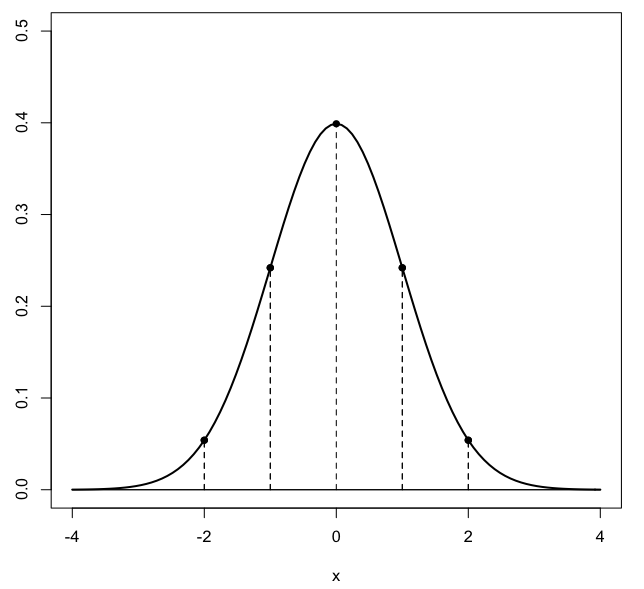
\includegraphics [scale=0.4] {gauss3.png} \end{center}
\begin{document}
\maketitle
\Large

The theory of complex functions
\[ f(z) \ \ \  z \in \mathbb{C} \]
is often described as being very beautiful.

It also makes possible the solution of many difficult integrals (over the real numbers).  Marsden gives three examples that he says are either very difficult or impossible if we cannot use complex integrals:
\[ \int_0^{\infty} \frac{\sin^2 x}{x^2} \ dx = \frac{\pi}{2} \]
\[ \int_0^{\infty} \frac{x^{\alpha-1}}{1+x} \ dx = \frac{\pi}{\sin \alpha \pi} \]
\[ \int_0^{2 \pi} \frac{d \theta}{a + \sin \theta} = \frac{2 \pi}{\sqrt{a^2-1}} \]

In this section we'll start by looking at some simpler complex functions---if you can just ignore the contradiction.

A complex function is a function whose input is a complex number $z$, an \emph{ordered pair} of two real numbers $x$ and $y$.  $f(z)$ generates or emits a second complex number which we may call $w$.
\[ w = f(z) = u(x,y) + i v(x,y) \]

The real part of $w$ is the output of $u(x,y)$, as the notation says.  $u(x,y)$ is a function of both $x$ and $y$, and similarly the imaginary part of $w$ is the output of $v(x,y)$.  The two functions $u$ and $v$ are real functions of two real variables.

Part of the "complexity" of complex functions is the multiple values of arguments ($\theta = \theta + 2 \pi$, and so on), but another part is that the calculus of complex functions is not like calculus of real functions.

We're used to thinking of the derivative as a slope, but for complex functions there is no simple geometric interpretation.  The derivative \emph{maps} $z$ to a new complex number. 

We compute the derivative of a real function as
\[ \frac{df}{dx} = \lim_{h \rightarrow 0} \frac{f(x+h) - f(x)}{h} \]
provided the limit exists.

In "approaching" $x$ or considering $x+h$ there are only two directions, from above (values $> x$), and from below (values $< x$).

For a complex function $f(z)$ which produces a complex number $w = f(z)$, the basic definition of the derivative is the same, but the crucial point is that we may approach $z$ in the Argand plane from any one of an infinite number of directions.  The resulting change in $f(z)$ --- the derivative --- must then be the same for \emph{all} of them.  

Not all functions have this property.  Those that do are called \emph{analytic}.

\begin{center} 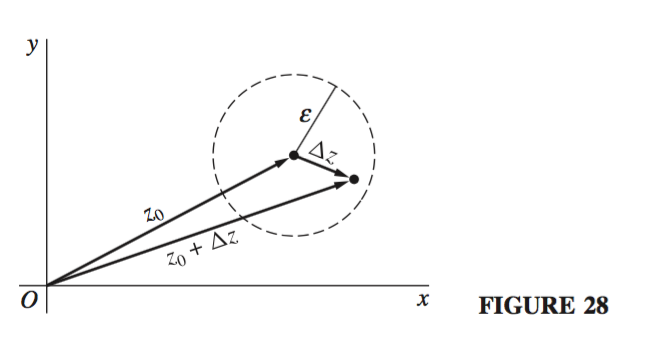
\includegraphics [scale=0.6] {Brown28.png} \end{center}
As we'll see later, if (and only if) the partial derivatives meet these conditions (called the CRE conditions):
\[ u_x = v_y \]
\[ u_y = - v_x \]
then the function in question is said to be analytic.

[The technical definition of an analytic function, or analyticity, is somewhat different but this property follows from it.  We don't need to worry about the distinction.]

An analytic function is differentiable, in other words, it's a good function and we can do calculus with it.  If a complex function is analytic, its derivative exists:  its value is independent of the direction in which change occurs.

So for example if we change a little bit in the $x$ direction, parallel with the real axis ($\Delta y = 0$), we get:
\[ f'(z) = u_x + iv_x  \]

Suppose
\[ f(z) = z^2 \]
\[ = (x + iy)(x + iy) \]
\[ = x^2 - y^2 + i2xy \]
Then
\[ u(x,y) = x^2 - y^2 \]
\[ v(x,y) = 2xy \]
So
\[ f'(z) = u_x + iv_x \]
\[ = 2x + i2y \]
\[ = 2(x + iy) =  2z \]
which should not be surprising.

Note that 
\[ f'(z) \ne u_y + i v_y \]
Instead
\[ f'(z) = v_y - i v_x \]
The basic reason is the chain rule.  We will see the reason for this shortly.

However, the ability to differentiate $f(z)$ here depends on the fact that $z^2$  is an analytic function (in fact, all powers of $z$ are analytic).

There are a few functions that are important and not analytic.  These can generally be seen to involve the complex conjugate:
\[ |z|^2 = zz* \]

For functions that have a derivative everywhere (excepting points where the function may vanish, like the origin for $1/z$), most of the usual rules of calculus apply
\[ \frac{d}{dz} c = 0, \ \ \  \text{where $c$ is a constant} \]
\[ \frac{d}{dz} z = 1 \]
\[ \frac{d}{dz} z^n = nz^{n-1}, \ \ \ n \ne 0 \]
\[ (f + g)' = f' + g' \]
\[ (fg)' = f' g + f g' \]
\[ (\frac{f}{g})' = \frac{f' g - f g'}{g^2} \]

\subsection*{exponential}
For a non-trivial introduction to using the CRE, we will explore the complex exponential function $f(z) = e^z$.  First of all, write
\[ e^z = e^{x + iy} \]
\[ = e^x e^{iy} \]
We can thus visualize the complex exponential as resulting in a number $w$ with modulus $e^x$ and argument $y$.

Reversing Euler:
\[ = e^x (\cos y + i \sin y) \]
\[ = e^x \cos y + i e^x \sin y \]
So the real part of $e^z$ is 
\[ u(x,y) = e^x \cos y \]
with partial derivatives:
\[ u_x = e^x \cos y \]
\[ u_y = - e^x \sin y \]
and the imaginary part is
\[ v(x,y) = e^x \sin y \]
with partials:
\[ v_x = e^x \sin y \]
\[ v_y = e^x \cos y \]
Hence
\[ u_x = v_y \]
\[ u_y = - v_x \]
The CRE conditions are satisfied and the complex exponential $e^z$ is analytic.  (Which, according to Shankar, we could have predicted, since it depends only on $z$ and not on $z*$).

Notice also that, evaluating the derivative along $\Delta y =0$:
\[ f'(z) = u_x + iv_x  \]
\[ = e^x \cos y + i e^x \sin y = z \]
The complex exponential is its own derivative.

Which is good because we want our definitions for the complex functions to give the standard results when $z$ has only a real part, i.e. when $y=0$.

Now, once more we recall Euler's formula (for a real variable $\theta$ or $x$):
\[ e^{i \theta} = \cos \theta + i \sin \theta \]
\[ e^{i x} = \cos x + i \sin x \]
Substitute $-x$ for $x$:
\[ e^{-i x} = \cos -x + i \sin -x \]
\[ = \cos x - i \sin x \]
By addition and subtraction we obtain:
\[ 2 \cos x = e^{i x} + e^{-i x} \]
\[ \cos x = \frac{e^{i x} + e^{-i x}}{2} \]
and
\[ 2i \sin x = e^{i x} - e^{-i x} \]
\[ \sin x = \frac{e^{i x} - e^{-i x}}{2i} \]
These can be taken as the \emph{definitions} of the complex sine and cosine.

We will also need the hyperbolic sine and cosine later so let's just remind ourselves:
\[ 2 \cosh x = e^x + e^{-x} \]
\[ 2 \sinh x = e^x - e^{-x} \]

As mentioned, the derivative of the complex exponential is as we would hope and expect:
\[ \frac{d}{dz} e^z = e^z \]

This can also be proved by using a Taylor series.  Shankar says to define $e^z$ in the same way as $e^x$.  That is, for real $x$:
\[ e^x = \sum_0^{\infty} \frac{x^n}{n!} \]
which we know converges because
\[ |x| < R = \lim_{n \rightarrow \infty} \frac{|a_n|}{|a_{n+1}|} \]
where $a_n = 1/n!$.  So
\[ e^z = \sum_0^{\infty} \frac{z^n}{n!} \]
and again we see that 
\[ \frac{d}{dz} \ e^z = e^z \]
differentiating the series term by term.

The complex exponential 
\[ e^z = e^x e^{iy} \]
has some properties that are not shared with the real exponential.  As we saw before, the angle $\theta + 2 \pi = \theta$, so any number is really a family of numbers with different $\theta + 2 \pi k$ for integer $k$.

In particular, $e^z$ is periodic with a period of $2 \pi i$.  Additionally, it is possible for $e^z$ to be negative.  
\subsection*{example:  exp(z) = -1}
Let us find $z$ such that:
\[ e^z = -1 \]
This corresponds to the point $(-1,0)$.  The simplest way is to use polar coordinates.  We can see that the length is $r = 1$, and the angle $\theta$ is equal to $\pi$.  So the number is
\[ 1 \cdot e^{i\pi} = e^{i\pi} = -1 \]
Going through $x$ and $y$:  let $z = 0 + i\pi$.  Then 
\[ e^x = e^0 = 1 \]
and
\[ e^{iy} = e^{i\pi} = -1 \]
So
\[ e^z = e^x e^{iy} = e^x(\cos y + i \sin y) = 1 (-1) = -1 \]
\subsection*{example: exp(z) = i}
This corresponds to the point $(0,1)$.  We can see (again) that the length is $r = 1$, and the angle is equal to $\pi/2$.  So the number is
\[ e^{i \cdot \pi/2} = i \]
\subsection*{non-zero}
On the other hand, $e^z$ \emph{cannot be zero}.
\[ e^z = e^x \cos y + i e^x \sin y = e^x(\cos y + i \sin y) \]
For $x \in \mathbb{R}$, $e^x > 0$ so the only way this could be zero would be if we can find a $y$ such that $\sin y$ and $\cos y$ were both zero.  Since there is no such $y$, we conclude that $e^z$ cannot be equal to zero.

\subsection*{derivation of the Cauchy-Riemann equations}
For a complex function $f(z)$ which produces a complex number $w = f(z)$, we may approach $z$ in the Argand plane from any one of an infinite number of directions.

The CRE are necessary and sufficient conditions such that the derivative is the same for any direction of approach.

Here are two quick proofs in the forward direction (differentiability implies the CRE):

Write the basic definition of the derivative of $f$ at the point $z_0$:
\[ f'(z_0) = \lim_{\Delta z \rightarrow 0} \frac{f(z + z_0) - f(z)}{\Delta z} \]
Now
\[ f'(z_0) =  \frac{dw}{dz} =   \lim_{\Delta z \rightarrow 0} \frac{\Delta w}{\Delta z} \]
\[ =  \lim_{\Delta z \rightarrow 0} \frac{\Delta u + i \Delta v}{\Delta x + i \Delta y} \]
Our constraint is that the derivative must be the same for any direction of approach.  

Pick two convenient directions:  with $\Delta y = 0$ or with $\Delta x = 0$.  For the first one, we have
\[ f'(z_0) = \lim_{\Delta z \rightarrow 0} \frac{\Delta u + i \Delta v}{\Delta x + i \Delta y} \]
\[ =  \lim_{\Delta x \rightarrow 0} \frac{\Delta u + i \Delta v}{\Delta x} \]
\[  =  \lim_{\Delta x \rightarrow 0} \frac{\Delta u}{\Delta x} + i \frac{\Delta v}{\Delta x} \]
Notice that $\Delta z \rightarrow 0$ becomes $\Delta x \rightarrow 0$ (because $\Delta y = 0$) and the limit is just equal to 
\[ f'(z_0) = u_x + i v_x \]
This is a standard limit for two real functions of two real variables.

For the second approach, with $\Delta x = 0$, we have
\[ f'(z_0) =  \lim_{\Delta y \rightarrow 0} \frac{\Delta u + i \Delta v}{i \Delta y} = \lim_{\Delta y \rightarrow 0} \frac{\Delta u}{i \Delta y} +  \frac{i \Delta v}{i \Delta y} \]
Here, the $i$ terms cancel on the right (and recall that $1/i = -i$) so we have:
\[ f'(z) = -i u_y + v_y \]
Equating the two results we have that 
\[ f'(z) = u_x + i v_x = v_y - i u_y \]
Both the real and the imaginary parts must be equal:
\[ u_x = v_y \]
\[ v_x = - u_y \]
These are the CRE.
\subsection*{alternative derivation}
Write:
\[ z = x + iy \]
Clearly,
\[ \frac{\partial z}{\partial x} = 1, \ \ \ \frac{\partial z}{\partial y} = i \]
Now,
\[ w = f(z) = u(x,y) + i \ v(x,y) \]
where $u$ and $v$ are real functions over $\mathbb{R}^2$.

Recalling the chain rule
\[ w = u(x,y) + i \ v(x,y) \]
\[ \frac{\partial w}{\partial x} = \frac{dw}{dz} \ \frac{\partial z}{\partial x} \]
\[ =  \frac{dw}{dz} \]
(by the result for $\partial z/\partial x$ immediately above).
Similarly
\[ \frac{\partial w}{\partial y} = \frac{dw}{dz} \ \frac{\partial z}{\partial y} \]
\[ =  i \frac{dw}{dz} \]
\[  \frac{dw}{dz} = -i \ \frac{\partial w}{\partial y} \]
Hence we can equate the two expressions 
\[ \frac{dw}{dz} = \frac{\partial w}{\partial x} = -i \frac{\partial w}{\partial y} \]

Now if we actually compute the partials
\[ \frac{\partial w}{\partial x} = u_x + i v_x \]
\[ \frac{\partial w}{\partial y} = u_y + i v_y \]
and plug them in to the previous equation, we obtain:
\[ u_x + i v_x = -i (u_y + i v_y) = v_y - i u_y \]
Exactly as we obtained by the first approach.  And since both the real and the imaginary parts must be equal:
\[ u_x = v_y \]
\[ v_x = - u_y \]
These are the CRE, again.

The result above
\[ \frac{df}{dz} = \frac{\partial f}{\partial x} = - i \frac{\partial f}{\partial y} \]
is just saying that the derivative $df/dz$ can be computed with constant $y$, or constant $x$ or anything in between.  Take the first direction, constant $y$:
\[ \frac{df}{dz} = \frac{\partial f}{\partial x} = u_x + i v_x \]

From above
\[ u_x = e^x \cos y \]
\[ v_x = e^x \sin y \]
\[ \frac{df}{dz} = \frac{\partial f}{\partial x} =  e^x \cos y + i  e^x \sin y = z \]
Just like for $x \in \mathbb{R}$, where
\[ \frac{d}{dx} \ e^x = e^x \]
For a $z \in \mathbb{C}$
\[ \frac{d}{dz} \ e^z = e^z \]

\subsection*{polar coordinates}

An alternative form of the CRE holds in polar coordinates:
\[ r u_r = v_{\theta} \]
\[ u_{\theta} = - r v_r \]

One way to get this is to write
\[ \frac{\partial u}{\partial r} =  \frac{\partial u}{\partial x}\frac{\partial x}{\partial r} + \frac{\partial u}{\partial y}\frac{\partial y}{\partial r} \]
and since 
\[ z = x + iy \]
\[= r \cos \theta + r \sin \theta \]
then using the equation with the partials and computing $x_r$, $y_r$ etc.:
\[ u_r = u_x x_r + u_y y_r \]
\[ u_r = u_x \cos \theta + u_y \sin \theta \]
while
\[ u_{\theta} = u_x x_{\theta} + u_y y_{\theta} \]
\[ u_{\theta} = -u_x \ r \sin \theta + u_y \  r \cos \theta \]
similarly
\[ \frac{\partial v}{\partial \theta} =  \frac{\partial v}{\partial x}\frac{\partial x}{\partial \theta} + \frac{\partial v}{\partial y}\frac{\partial y}{\partial \theta} \]
\[ v_{\theta} = -v_x \ r \sin \theta + v_y \ r \cos \theta \]
while
\[ v_r = v_x x_r + v_y y_r \]
\[ v_r = v_x \cos \theta + v_y \sin \theta \]

Substituting from the cartesian CRE, rewrite the last equation as
\[ v_r = -u_y \cos \theta + u_x \sin \theta \]
multiply by $r$
\[ r v_r = -u_y \ r \cos \theta + u_x \ r \sin \theta = - u_\theta  \]
This is the second of the polar form CRE as given above. Similarly
\[ u_r = u_x \cos \theta + u_y \sin \theta \]
substituting
\[ u_r = v_y \cos \theta + - v_x \sin \theta \]
\[ r u_r = v_y \ r \cos \theta + - v_x \ r \sin \theta = v_{\theta} \]
which is the other one.

\subsection*{trig functions}
We can define the complex counterparts of the real trigonometric functions similarly to their real equivalents by saying that Euler's formula is also good for a complex number $z$ (a math book would define them by their power series).  So
\[ e^{iz} = \cos z + i \sin z \]
\[ e^{-iz} = \cos -z + i \sin -z = \cos z - i \sin z \]
This leads to:
\[ e^{iz} + e^{-iz} = 2 \cos z \]
and
\[ e^{iz} - e^{-iz} = 2i \sin z \]

On the other hand, Shankar defines them using series in the same way as the real versions:
\[ \sin z = \sum_0^{\infty} (-1)^n \frac{z^{2n+1}}{(2n +1)!} \]
\[ \cos z = \sum_0^{\infty} (-1)^n \frac{z^{2n}}{(2n)!} \]
\[ \sinh z = \sum_0^{\infty} \frac{z^{2n+1}}{(2n +1)!} \]
\[ \cosh z = \sum_0^{\infty} \frac{z^{2n}}{(2n)!} \]
and showing that they converge for any $z$.

A nice property for this definition of cosine is that
\[ \cos z = \frac{1}{2} \ (e^{iz} + e^{-iz}) \]
so
\[ \cos (z + 2\pi) = \frac{1}{2} \ (e^{iz}e^{i2\pi} + e^{-iz}e^{-2\pi}) \]
but
\[ e^{i 2 \pi} = \cos 2 \pi + i \sin 2 \pi = 1 = e^{-i 2 \pi} \]
so
\[ \cos (z + 2\pi) = \cos z \]
The \emph{period} of the complex cosine (and the complex sine) is $2 \pi$.

Take derivatives
\[ \cos z = \frac{1}{2} \ (e^{iz} + e^{-iz} ) \]
\[ \frac{d}{dz} \ \cos z = \frac{1}{2} \ (i e^{iz} - i e^{-iz} ) \]
\[ = \frac{i}{2} \ 2i \sin z = -\sin z \]
Similarly
\[ \sin z = \frac{1}{2i} \ (e^{iz} - e^{-iz}) \]
\[ \frac{d}{dz} \ \sin z = \frac{1}{2i} i (e^{iz} + e^{-iz}) = \cos z \]
\subsection*{hyperbolic connection}
\[ \cos z = \frac{e^{iz} + e^{-iz}}{2} \]
if we consider $z = iy$ then
\[ \cos iy = \frac{e^{i^2y} + e^{-i^2y}}{2} \]
\[ = \frac{e^{-y} + e^{y}}{2} \]
But this is just $\cosh y$.  That is:
\[ \cos iy = \cosh y \]
Similarly
\[ 2i \sin iy = e^{i^2y} - e^{-i^2y} \]
\[ = e^{-y} - e^{y} \]
\[ = - (e^y - e^{-y}) \]
\[ = -2 \sinh y \]
Hence 
\[ i \sin i y = -\sinh y \]
\[ \sin i y =  i \sinh y \]
So what this means is that
\[ \cos z = \cos (x + iy) \]
By the angle addition formula:
\[ = \cos x \cos i y - \sin x \sin i y \]
\[ = \cos x \cosh y - i \sin x \sinh y \]
and what's nice about this is that we have the real and imaginary parts of the complex cosine easily visible.  Similarly
\[ \sin z = \sin(x + iy) \]
\[ = \sin x \cos iy + \cos x \sin iy \]
\[ = \sin x \cosh y + i \cos x \sinh y \]

\subsection*{analyticity}
We proved above that the complex exponential is analytic.  There is a theorem that says that if we add two analytic functions together, the result is also analytic.  Hence, the trigonometric functions are analytic.

But, just to check this result, let's write them out in terms of $u$ and $v$ and see whether the partial derivatives follow the CRE conditions:
\[ \sin z = \sin(x + iy) \]
Again, by the addition formula
\[ \sin z = \sin x \cos iy + \sin iy \cos x \]
where $x$ and $y$ are real.

Recalling the result for the hyperbolic sine and cosine from above
\[ \cos iy = \cosh y \]
\[ \sin i y =  i \sinh y \]
then
\[ \sin z = \sin x \cos iy + \sin iy \cos x \]
\[ = \sin x \cosh y + i \cos x \sinh y \]
Taking the derivatives:
\[ u(x,y) =  \sin x \cosh y \]
\[ u_x = \cos x \cosh y \]
\[ u_y = \sin x \sinh y \]
and
\[ v(x,y) = \cos x \sinh y \]
\[ v_x = - \sin x \sinh y \]
\[ v_y = \cos x \cosh y \]
So we see that
\[ u_x = v_y \]
\[ u_y = -v_x \]

The CRE are satisfied and therefore, the complex sine is analytic.

Similarly we have that 
\[ \cos z = \cos (x + iy) \]
\[ = \cos x \cos iy - \sin x \sin iy \]
\[ = \cos x \cosh y - i \sin x \sinh y \]
So
\[ u(x,y) =  \cos x \cosh y \]
\[ u_x = - \sin x \cosh y \]
\[ u_y = \cos x \sinh y \]
and
\[ v(x,y) = -\sin x \sinh y \]
\[ v_x = -\cos x \sinh y \]
\[ v_y = -\sin x \cosh y \]
So we see that
\[ u_x = v_y \]
\[ u_y = v_x \]
Thus the complex cosine is also analytic.

We can also prove that:

\[ \sin^2 z + \cos^2 z = 1 \]
The easy way is
\[ \cos^2 z + \sin^2 z = \ [ \frac{e^{iz} + e^{-iz}}{2} \ ]^2 +  [ \frac{e^{iz} - e^{-iz}}{2i} \ ]^2 \ ] \]
\[= \frac{e^{2iz} + 2 + e^{-2iz} - e^{2iz} + 2 - e^{-2iz} }{4} \]
\[ = 1 \]

\subsection*{logarithm}

Nearly everything works for $z$ similarly to the real numbers, except for the issue of multiple phase angles or complex arguments.  For example
\[ \log(z) = \log(re^{i\theta}) = \ln r + i \theta \]
but we may have any multiple of $2 \pi n$ added to $\theta$
\[ \log(z) = \ln r + i (\theta + 2 \pi n) \]
We call one particular range of $2 \pi$ the range for the principal value of the function.  

For example, here it is natural to make the range go from $-\pi < \theta < \pi$.  The reason is that the negative $x$-axis consists of negative real numbers, for which the natural logarithm isn't defined, and neither is the complex logarithm.  So we exclude that from the domain of the complex logarithm.  This is called a "branch cut," and we take one particular branch of this multi-valued function.

Here is a derivation.  
\[ z = x + iy = re^{i\theta} = r(\cos \theta + i \sin \theta) \]
\[ r = |z| = \sqrt{x^2 + y^2} \]

The logarithm of $z$ is $w$
\[ w = \log z \iff e^w = z \]
So what about $w$? Well, in general, it's a complex number
\[ w = u + iv \]
so
\[ e^w = e^{u + iv} = e^u (\cos v + i \sin v) \]
Equating the two we get
\[ r (\cos \theta + i \sin \theta) = e^u (\cos v + i \sin v) \]
Hence
\[ u = \ln r \]
\[ v = \theta \]
So
\[ w = \ln r + i \theta \]
\subsection*{change to a different base}
What is 
\[ i^i = \  ? \]
So the complex logarithm of $i$ is
\[ \log i = \ln r + i \theta = \ln 1 + i \frac{\pi}{2} =  i \frac{\pi}{2} \]
 Write
\[ a^z = (e^{\log a})^z \]
\[ i^i = (e^{\log i})^i = (e^{i \pi/2})^i = e^{-\pi/2} \]
Not only is $i$ to the $ith$ power computable, it is entirely real.  The value is $\approx 0.2079$.
\subsection*{derivative}
When we studied the Cauchy-Riemann equations we showed that if $f(z)$ is differentiable, then the CRE hold.  The converse theorem is also true, that if the CRE hold, then $f(z)$ is differentiable, and its derivative is
\[ f'(z) = \frac{\partial u}{\partial x} + i \frac{\partial v}{\partial x} \]

So we have that the logarithm function is
\[ \log(z) = \ln |z| + i \theta \]
Rewriting in terms of $x$ and $y$ we have that
\[ \log (x+iy) = \ln (\sqrt{x^2 + y^2}) + i \tan^{-1} (\frac{y}{x}) \]
\[ \log (x+iy) = \frac{1}{2} \ln (x^2 + y^2) + i \tan^{-1} (\frac{y}{x}) \]
So
\[ u(x,y) = \frac{1}{2} \ln (x^2 + y^2) \]
\[ u_x = \frac{1}{2} \ \frac{2x}{x^2 + y^2} = \frac{x}{x^2 + y^2} \]
\[ u_y = \frac{y}{x^2 + y^2} \]
and 
\[ v(x,y) = \tan^{-1} (\frac{y}{x}) \]
\[ v_x = \frac{1}{1 + (y/x)^2} \ y \ (-\frac{1}{x^2}) = \frac{-y}{x^2 + y^2} \]
\[ v_y = \frac{1}{1 + (y/x)^2} \ \frac{1}{x} = \frac{x}{x^2 + y^2} \]
We see that CRE are satisfied and this means that the derivative is
\[ \ [ \ \log z \ ] ' \ = u_x + i v_x \]
\[ = \frac{x}{x^2 + y^2} + i \frac{-y}{x^2 + y^2} \] 
\[ = \frac{1}{x^2 + y^2} (x - i y) \]
\[ = \frac{1}{|z|^2} \ z* \]
\[ =  \frac{1}{zz*} \ z* = \frac{1}{z} \]
The derivative of the complex logarithm is the inverse of $z$, analogous to the real case.

\end{document} 